\documentclass[12pt]{ctexart}

\usepackage{geometry}
\usepackage{booktabs}
\usepackage{graphicx}
\usepackage[final]{pdfpages}
\usepackage[stable]{footmisc}
\usepackage{threeparttable}
\usepackage{indentfirst}
\usepackage{minted}
\usepackage{listings}
\usepackage{xcolor}
\usepackage{subfigure}
\usepackage{amsmath}
\usepackage{amsfonts}
\usepackage{hyperref}
\usepackage{cleveref}
\crefformat{figure}{#2图~#1#3}
\crefrangeformat{figure}{图~(#3#1#4)\;\~{}\;(#5#2#6)}
\crefmultiformat{figure}{图~(#2#1#3)}{和~(#2#1#3)}{,(#2#1#3)}{和~(#2#1#3)}

% \setlength{\parindent}{0pt}
\geometry{top=25mm,bottom=25mm,left=25mm,right=25mm}
\lstset{
    basicstyle=\tt,
    basicstyle=\small,
    keywordstyle=\color{purple}\bfseries,
    rulesepcolor= \color{gray},
    breaklines=true,
    numbers=left,
    numberstyle= \small,
    commentstyle=\color{gray},
    frame=shadowbox
}

\hypersetup{
    hypertex=true,
    colorlinks=true,
    linkcolor=blue,
    filecolor=magenta,      
    urlcolor=cyan,
    anchorcolor=blue,
    citecolor=blue
}

\urlstyle{same}

\title{广义递归(一)}
\author{杜睿、张伟志}

\begin{document}

\maketitle
\begin{abstract}
    开始,我们将从最经典的问题入手,了解如何首先形式化地命名建模,再基于直觉建立递归式,最后尝试求得递归式的闭式解(数学归纳法、递归树法、特征根法)。这些问题都曾被数学家们反复研究过,由于太过经典大家并不会感觉陌生。
    
    中途,我们将探讨一个具体的问题。这个具体问题是“3或5的倍数”的扩展版本,涉及辗转相除法、容斥原理,和广义递归、0-1背包、汉诺塔、分平面等经典问题也有关联。然后,大家要独立阅读三道题目并建立递归式。

    最后,我们将接触到另一个具体问题——峰值查找。在这个问题中,我们同样是考虑建立原问题与规模更小的子问题之间的联系进而求解,只不过递归模式略有不同(折半查找、分而治之)。
\end{abstract}

\section{汉诺塔}
给定一个由$N$个圆盘组成的塔,这些圆盘按照\emph{大小递减}的方式套在三根桩柱中的一根上。我们的目的是要将\emph{整个塔}移动到另一根桩柱上,并作要求:
\begin{enumerate}
    \item 每次只能移动一个圆盘;
    \item 较大的圆盘在移动过程中不能放置在较小的圆盘上面。
\end{enumerate}

问:要完成这项任务移动多少次才是\emph{必须且足够}的?\newline

提交链接:\url{https://www.luogu.com.cn/problem/T291125}

扩展阅读:汉诺四塔、Frame–Stewart算法

\newpage
Hint1: \textit{某个算法“足以”解决问题(suffice),意味着这个算法可以保证解决问题,但某个或某些步骤有可能是“多此一举”的;某些步骤是“必须”的(necessary),意味着如果再在此基础上减少其中任意一个步骤,均不能解决问题。}\newline

Hint2: \textit{Smart mathematicians 
are not ashamed to think small, 
because general patterns are easier to perceive when the extreme cases are well understood (even when they are trivial).
}\newline

Hint3: \textit{考虑搬动最大盘的“前夕”必然的格局情形。}



\newpage
\section{分平面}
问:平面上$N$条直线所界定的区域的最大个数$L_n$是多少?

\begin{figure}[htbp]
    \centering
    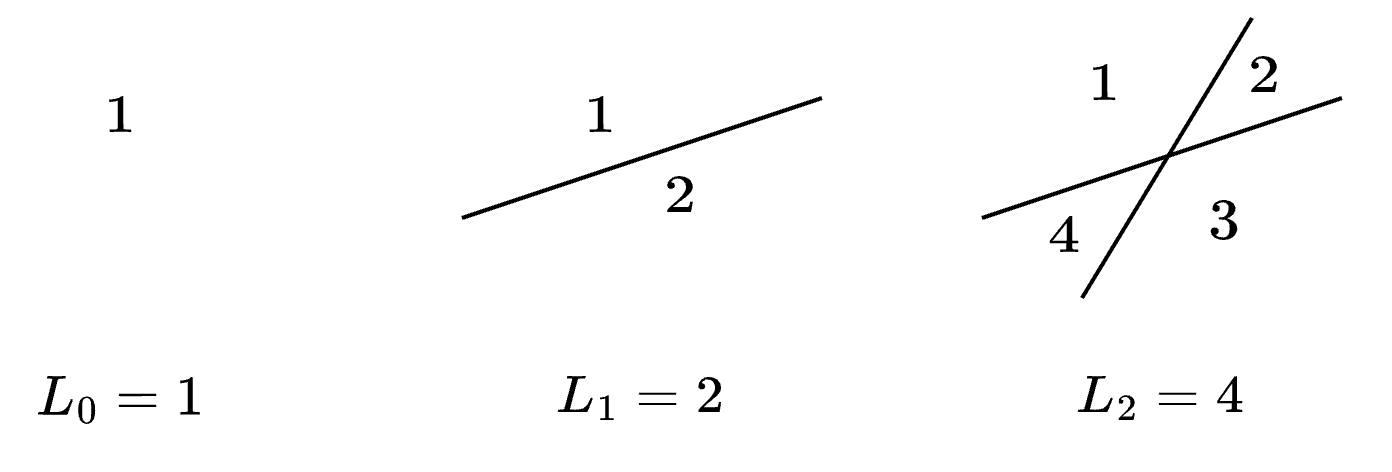
\includegraphics[width=0.65\linewidth]{assets/2-0.png}
\end{figure}

提交链接:\url{https://www.luogu.com.cn/problem/T291123}\newline

再问:由3个重叠的\textbf{圆}做成的维恩图常用来描述与3个给定集合有关的8个可能的子集。由4个给定集合给出的16种可能的子集能否用4个重叠的圆来描述?

\begin{figure}[htbp]
    \centering
    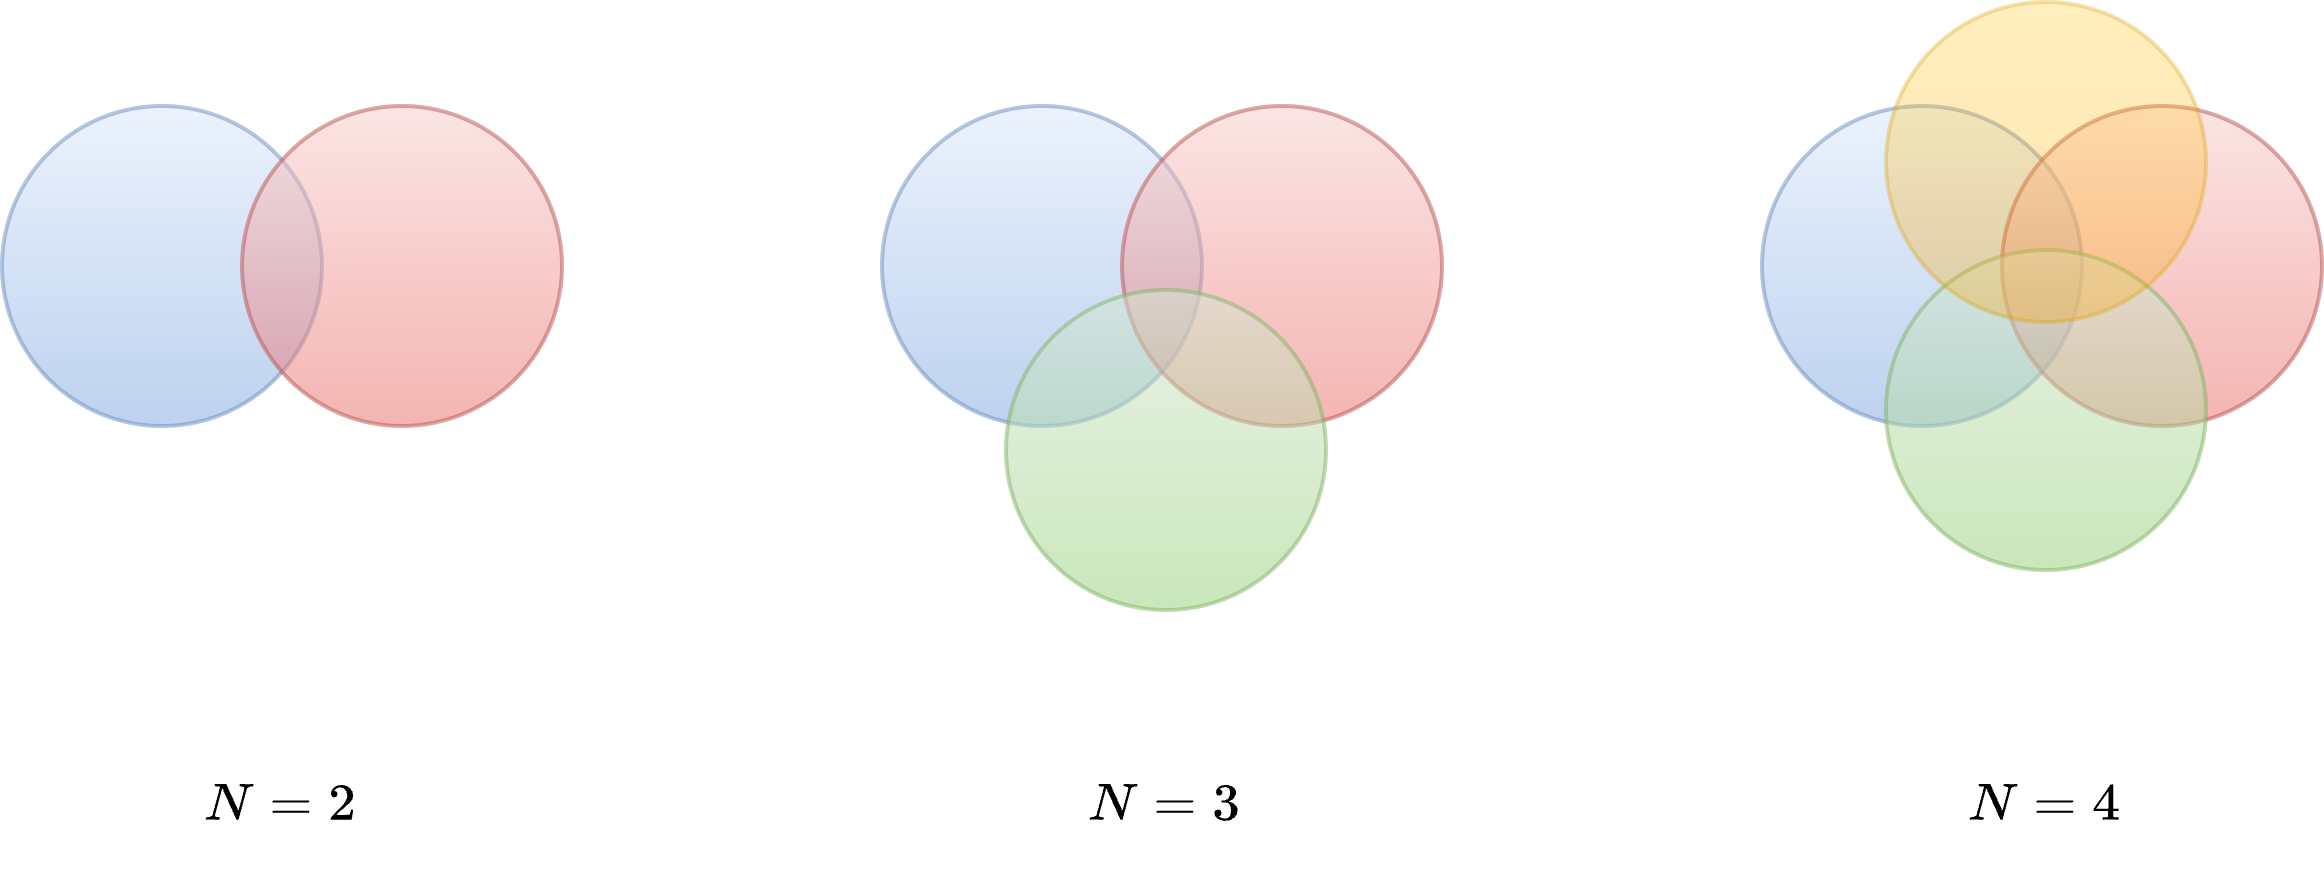
\includegraphics[width=0.85\linewidth]{assets/2-1.png}
\end{figure}

再问:假设我们用折线代替直线,每一条折线包含一个“锯齿”。平面上由$N$条这样折线所界定的区域的最大个数$Z_n$是多少?\newline

\begin{figure}[htbp]
    \centering
    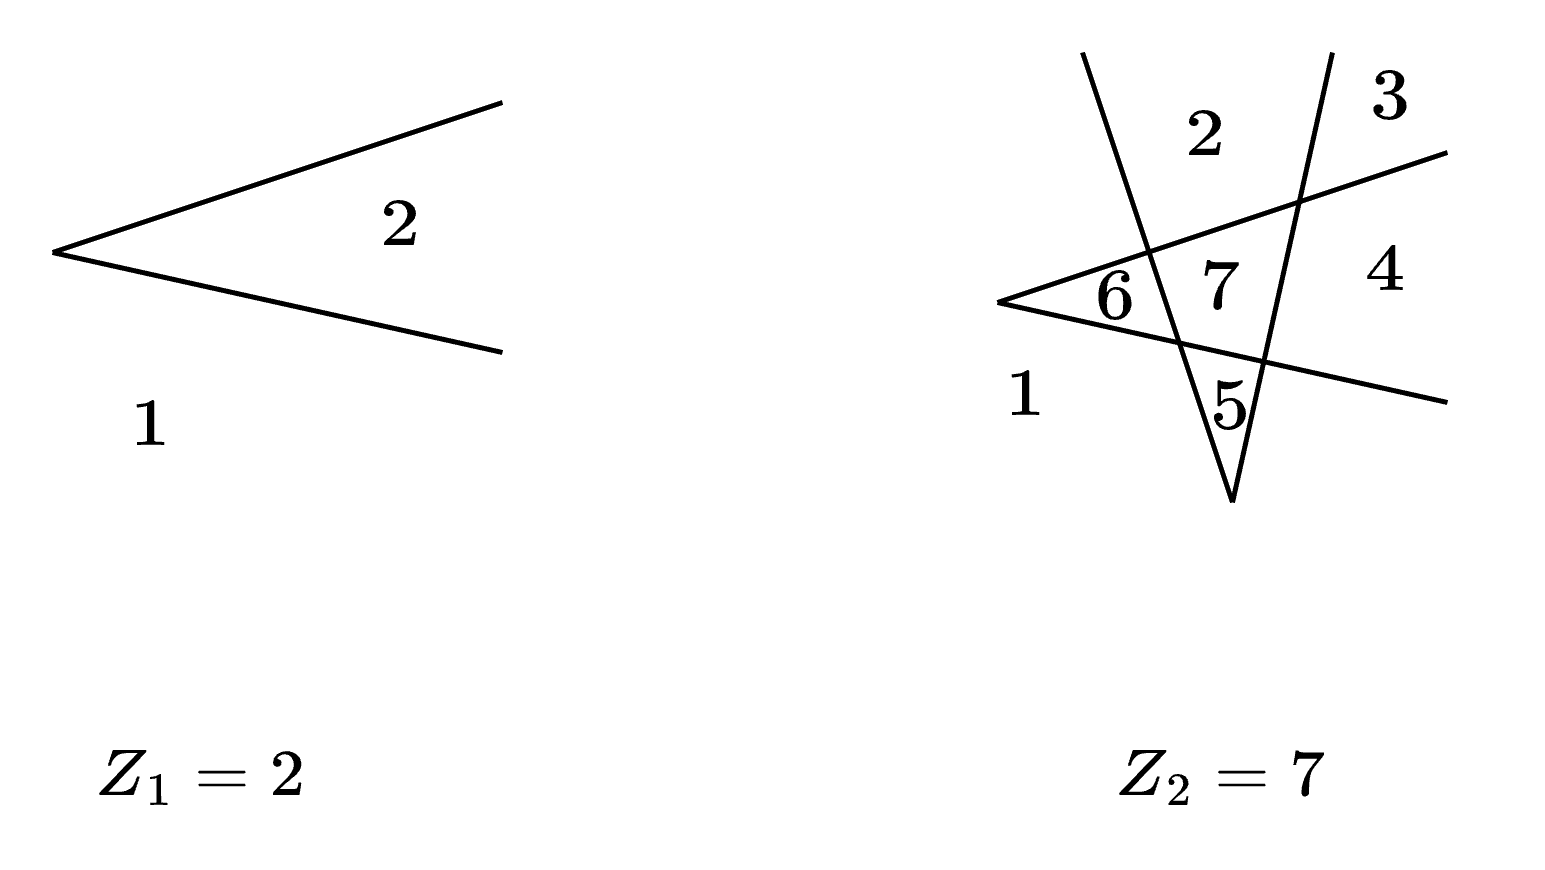
\includegraphics[width=0.55\linewidth]{assets/2-2.png}
\end{figure}

\newpage
Hint1: \textit{在$n$个顶点上的完全图被记作$k_n$,有$\frac{n(n-1)}{2}$条边。}\newline

Hint2: \textit{如下图。}


\begin{figure}[htbp]
    \centering
    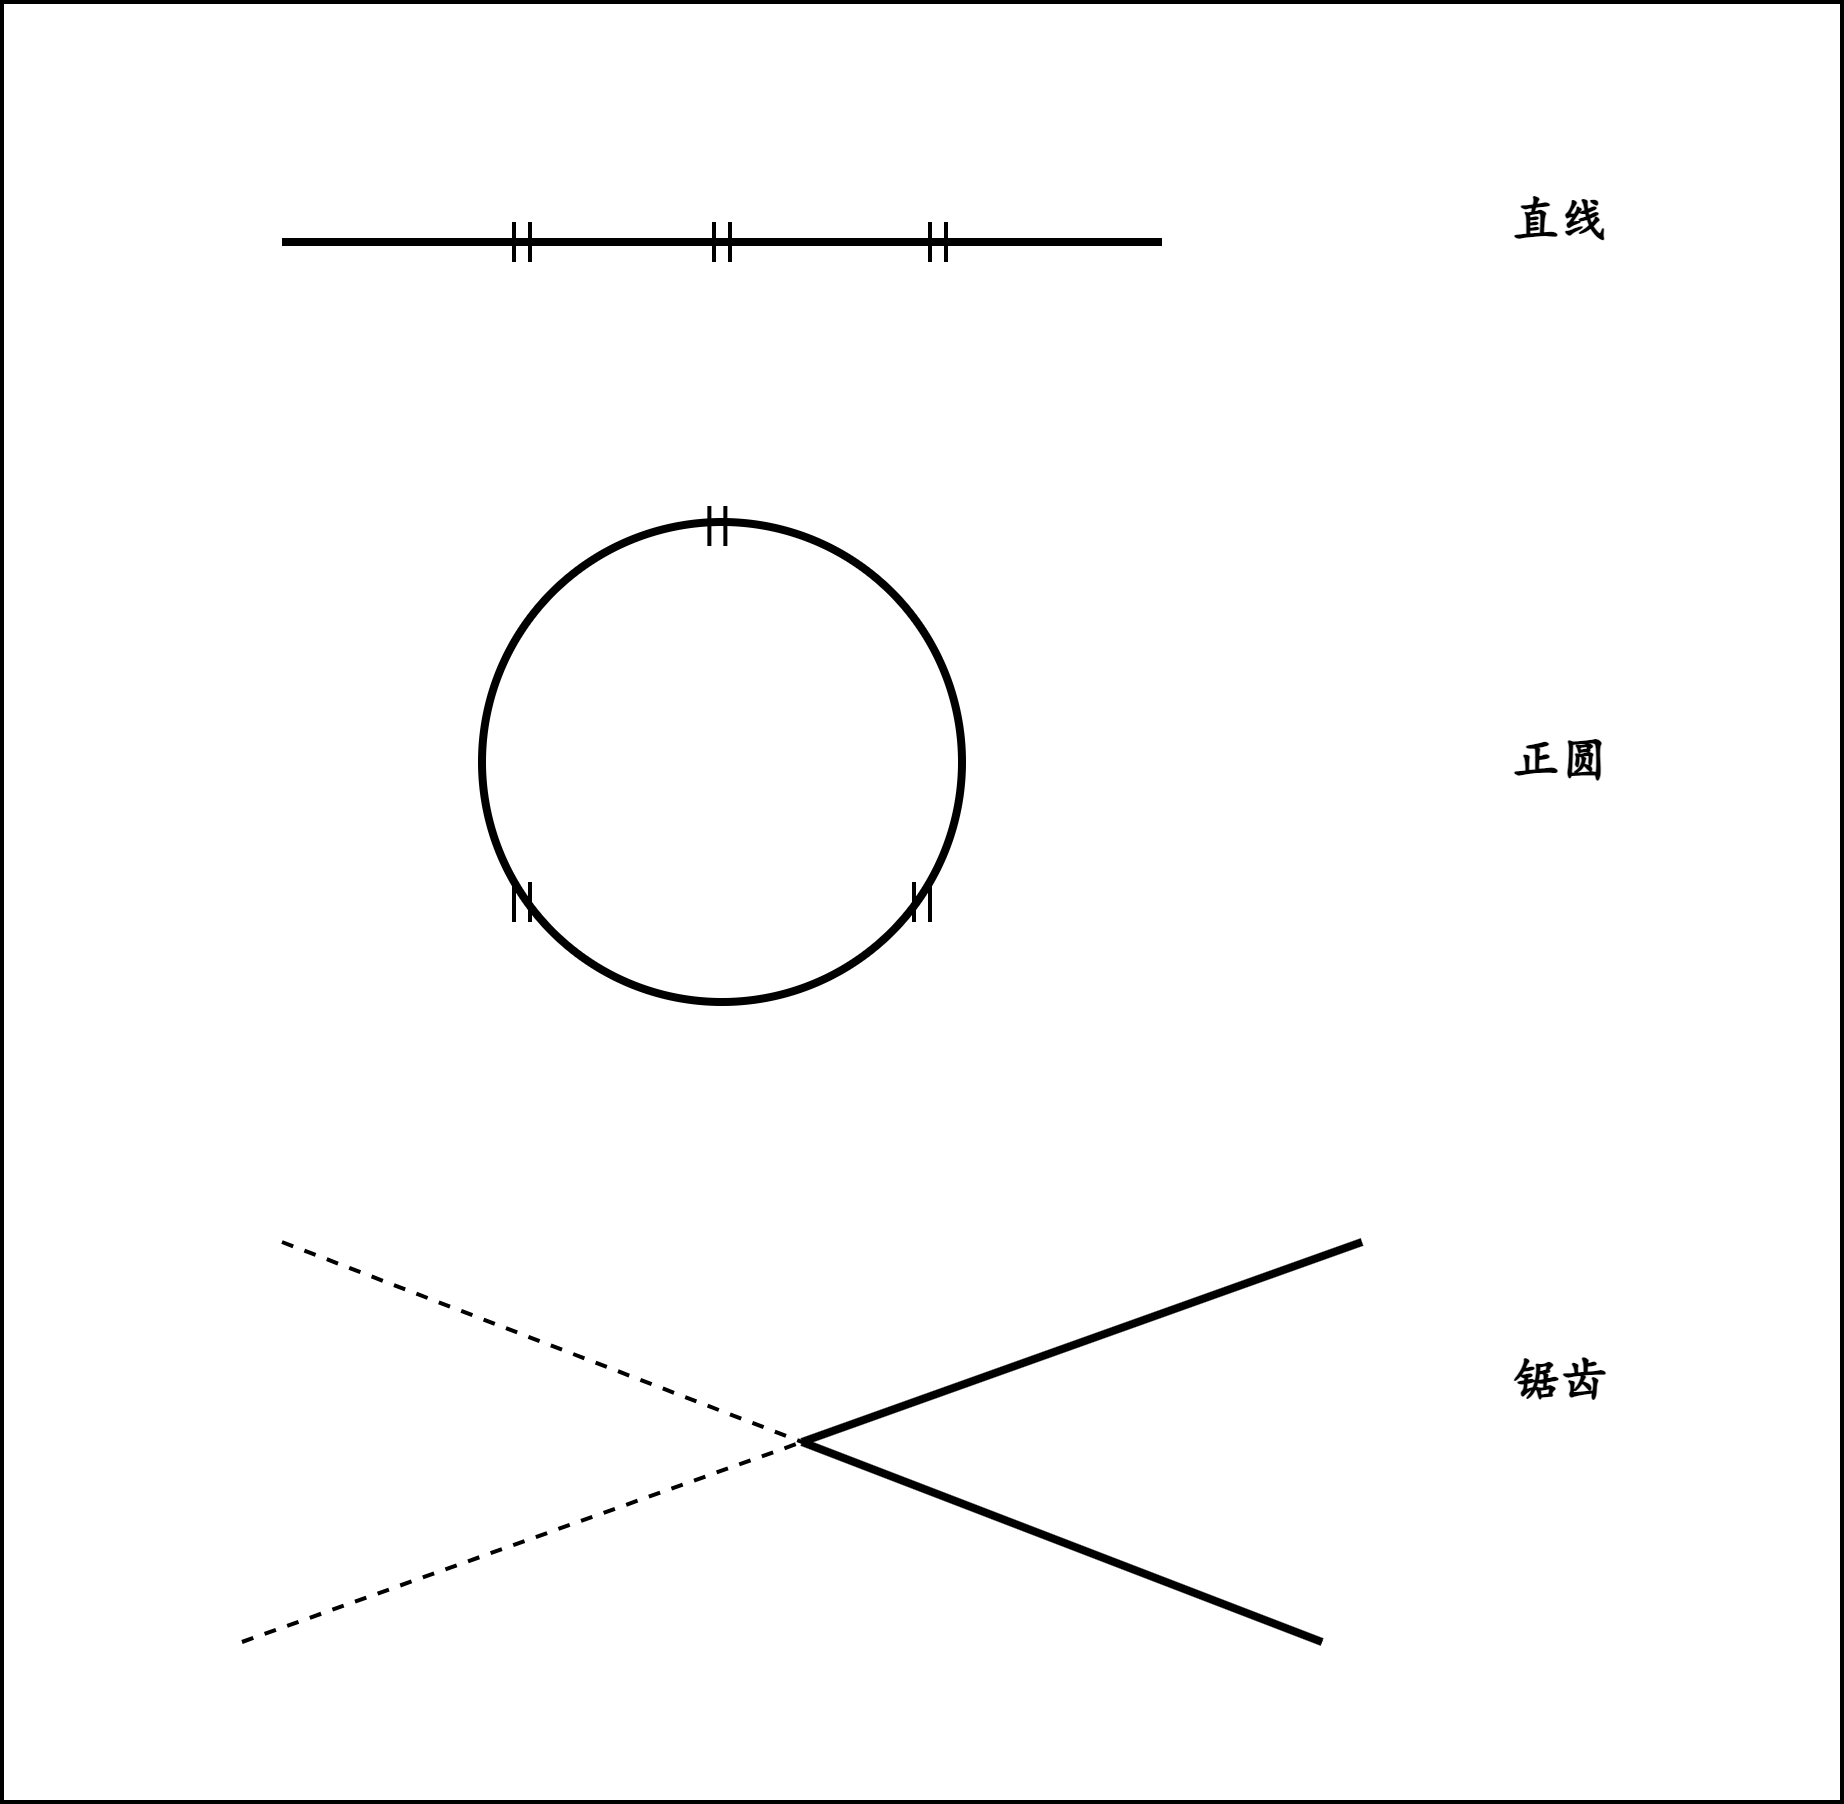
\includegraphics[width=0.75\linewidth]{assets/2-4.png}
\end{figure}




\newpage
\section{约瑟夫环}
$n$ 个人的编号是 $1 \sim n$,如果他们依编号按顺时针排成一个圆圈,从编号是 $1$ 的人开始顺时针报数。(报数是从 $1$ 报起)当报到 $k$ 的时候,这个人就退出游戏圈。下一个人重新从 $1$ 开始报数。问:幸存者的号码$J(n, k)$。\newline

\begin{figure}[htbp]
    \centering
    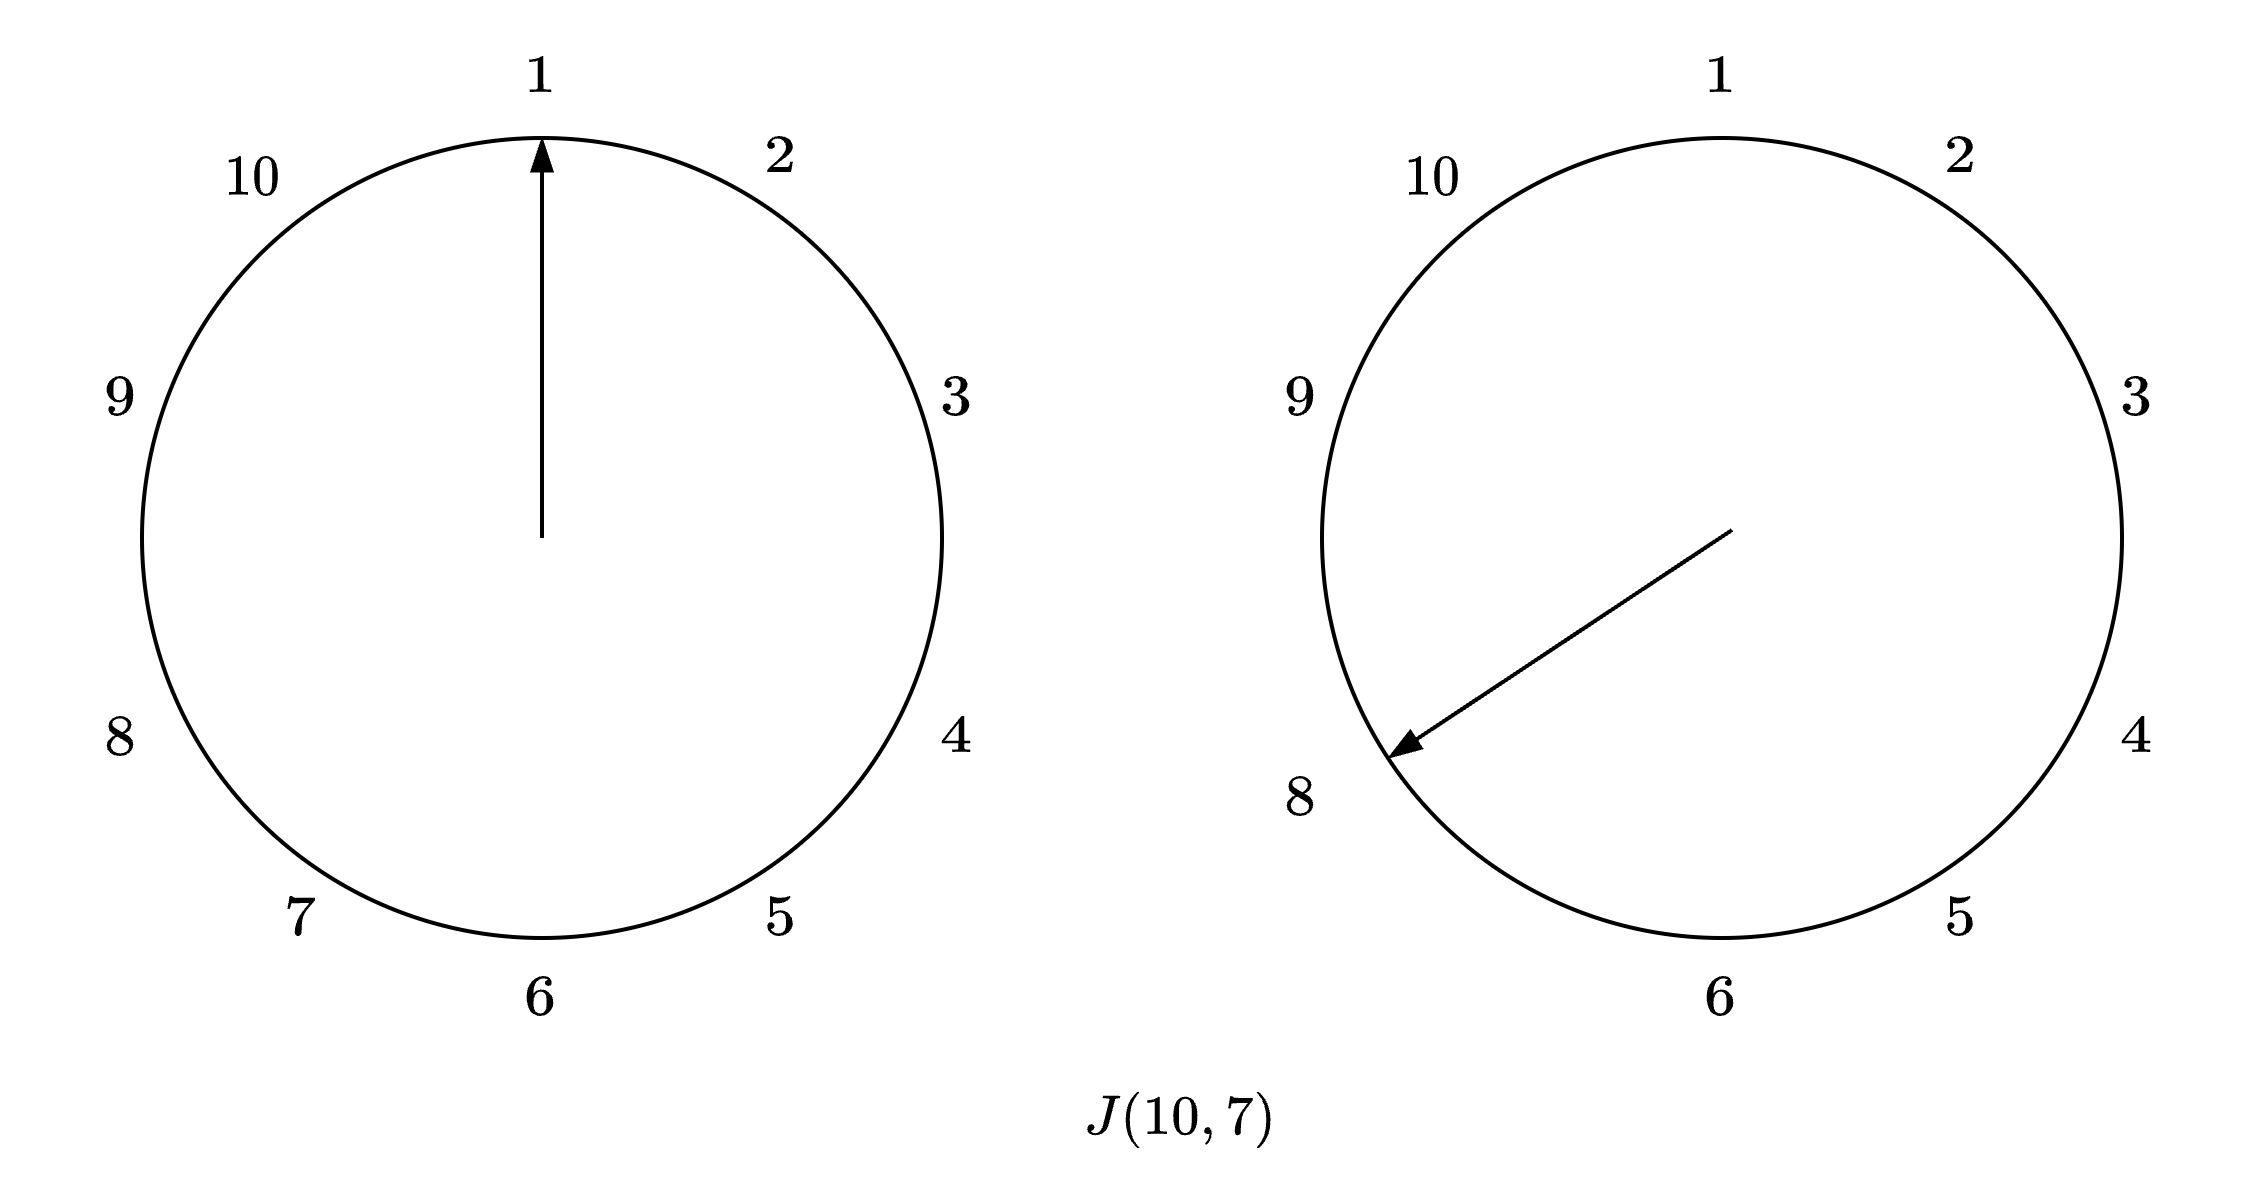
\includegraphics[width=0.8\linewidth]{assets/3-1.png}
\end{figure}

提交链接:\url{https://www.luogu.com.cn/problem/T291920}\newline

\newpage
Hint1: \textit{移一步,就是重映射一次下标。}\newline

Hint2: \textit{$mod(a+b, d) = mod(mod(a, d) + mod(b, d), d)$}\newline

Hint3: \textit{$[0, n-1] \rightarrow [1, n]$ }

\newpage
\section{罗马:能被整除的数}
给定一个正整数 $m$,以及 $n$ 个不同的正整数 $a_1, a_2, \dots, a_n$。

请你求出 $1 \sim m$ 中能被 $a_1, a_2, \dots, a_n$ 中的至少一个数整除的整数有多少个。\newline

提交链接:\url{https://www.luogu.com.cn/problem/U375671}

Keywords:质数分解唯一性,容斥原理,0-1背包、汉诺塔、圆分平面;最大公约数、最小公倍数、辗转相除法、更相减损术

\subsection{3或5的倍数}

假如给定一个正整数 $m$,以及 $n = 2$ 个不同的正整数 $3$, $5$。求 $1 \sim m$ 这$m$个数中是 $3$ 或 $5$ 的倍数的有几个。不难看出,是 $3$ 的倍数的有 $\lfloor \frac{m}{3} \rfloor$ 个,是 $5$ 的倍数的有 $\lfloor \frac{m}{5} \rfloor$ 个,一个天真的想法是将这两者加起来。然而,在 $1 \sim m$ 中存在这样的一系列的数,它既是 $3$ 的倍数又是 $5$ 的倍数,会被重复计算导致结果错误。

把上述问题推广到更一般的情况,在 $n$ 类事物计数时为了保证不重不漏,要引入容斥原理,表示为以下“奇加偶减”的形式:

$$|A_1 \cup A_2 \ldots A_n| = \sum_{1\le i\le n} |A_i| - \sum_{1\le i < j \le n} |A_i \cap A_j| + \sum_{1\le i < j < k \le n} |A_i \cap A_j \cap A_k|- \ldots + (-1)^{n+1} |A_1 \cap A_2 \cap \ldots \cap A_n|$$

其中$A_i$代表第$i$类事物(集合),$|A_i|$代表集合中元素个数。\newline

具体对“$3$或$5$的倍数”来说,$A_1$代表“是$3$的倍数的数”的集合,$A_2$代表“是$5$的倍数的数”的集合,$A_1 \cap A_2$ 也是一个集合,其中每个元素都既是$3$的倍数又是$5$的倍数,即是$3$和$5$公倍数,也就是$3$和$5$最小公倍数($15$)的倍数。\newline

对于两个正整数 $a$, $b$,根据“质数唯一分解定理”,不难得$a \times b = gcd(a, b) * lcm(a, b)$。求解最大公约数的经典算法有“辗转相除法”、“更相减损术”。它们均基于以下事实:

当$a\ge kb$时,$gcd(a, b) = gcd(a-kb, b)$,$k$为正整数。当$k$取最大值$\lfloor \frac{a}{b} \rfloor$时,又可以写成$gcd(a, b) = gcd(a\%b, b) = gcd(b, a \% b)$。

\newpage
\subsection{容斥原理}
\subsubsection{符号说明}
容斥原理在韦恩图中表现为每块最小区域只计算一次。为了方便,我们借用数字逻辑中函数、变元的概念,将每块最小区域视作如图的形式。从而,将容斥原理变相地表述为下面并不十分严谨的另一种形式,用以表示每块最小区域的计算次数:

\begin{figure}[htbp]
    \centering
    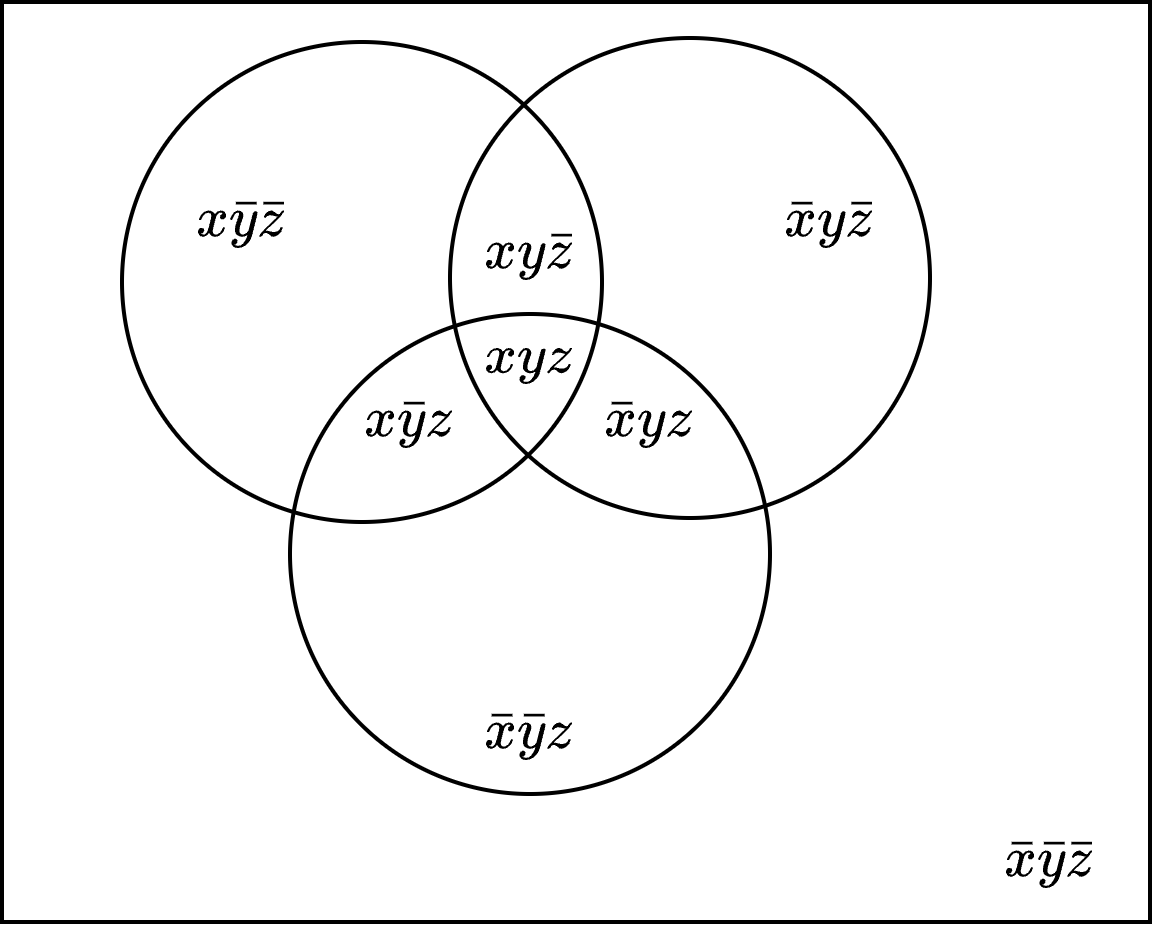
\includegraphics[width=0.55\linewidth]{assets/4-p.png}
\end{figure}



“类”最简与或式。:
$$G(x, y, z) = x + y + z - xy - yz - xz + xyz$$

“类”标准与或式:
$$
\begin{aligned}
    G(x, y, z) &= 1 - \bar{x}\bar{y}\bar{z} \\ 
    &= x\bar{y}\bar{z} + \bar{x}y\bar{z} + \bar{x}\bar{y}z + \bar{x}yz + xy\bar{z}  + x\bar{y}z + xyz
\end{aligned}
$$

\newpage
\subsubsection{启发:类标准与或式、0-1背包}
类标准与或式成立的一个必要条件是:

\begin{equation}\label{eq1}
\sum_{i=1}^{n} (-1)^{i+1} C_{n}^{i} \cdot 2^{n-i} = 2^{n} - 1
\end{equation}

\begin{itemize}
    \item 类标准与或式有$2^{n} - 1$项。
    \item 如\cref{img:001}~所示,在“奇加偶减”的指导原则下,正负抵消应有$\sum_{i=1}^{n} (-1)^{i+1} C_{n}^{i} \cdot 2^{n-i}$项。
\end{itemize}

\begin{figure}[htbp]
    \centering
    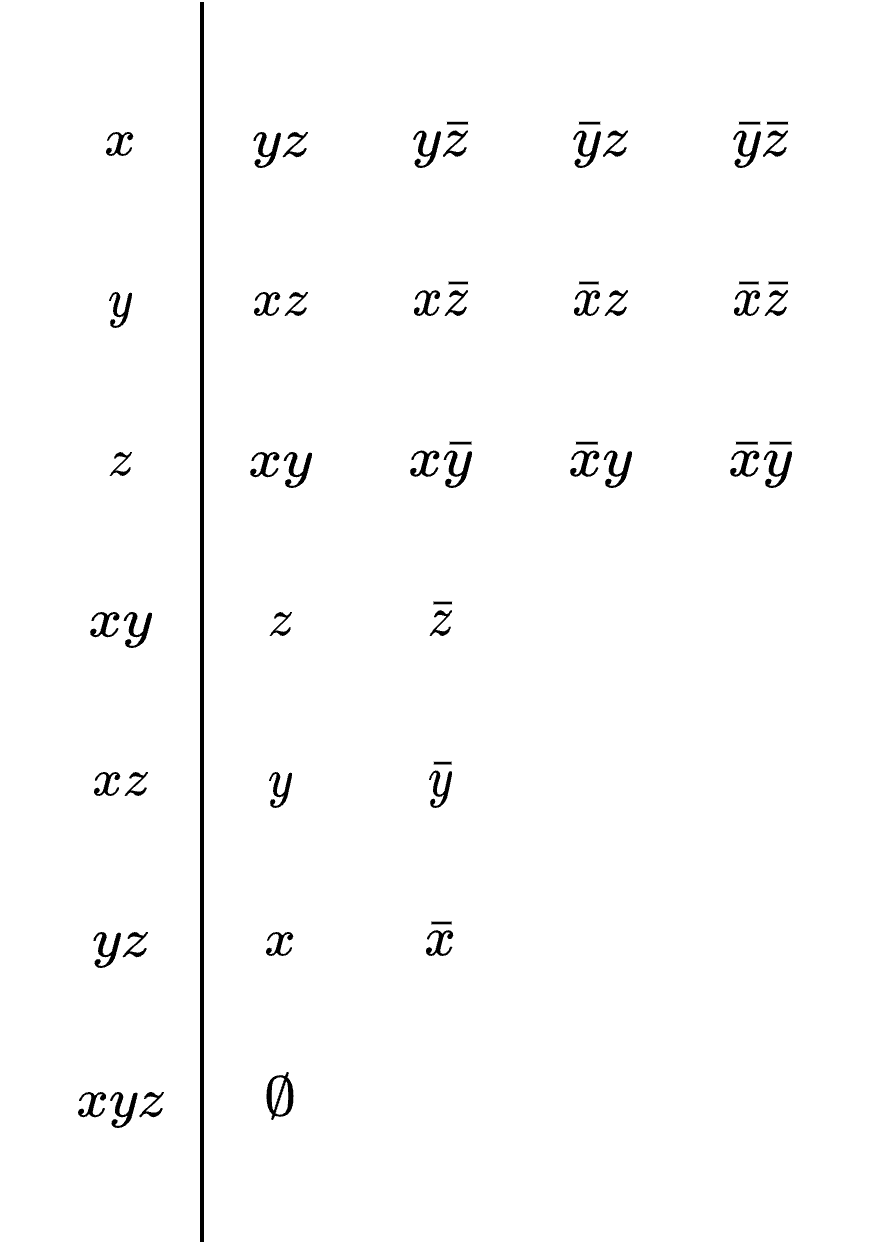
\includegraphics[width=0.35\linewidth]{assets/4-1.png}
    \caption{三问题变元的情况}
    \label{img:001}
\end{figure}

要证\eqref{eq1}式,即要证:

\begin{align}
    F(n) &= 1 + \sum_{i=0}^{n} (-1)^{i+1} C_{n}^{i} \cdot 2^{n-i} \\~ F(n) &= 0 
\end{align}

证明如下:

易证,$F(1)=0$;下面假设$F(n)=0$成立,转而要证$F(n+1)=0$。

\newpage
不妨先考虑$n$为偶数:

\begin{equation}
\begin{cases}
 F(n) &= 1 \textcolor{red}{- C_n^0 2^n + C_n^1 2^{n-1} - \cdots - C_n^{n-2} 2^{2} + C_n^{n-1} 2^{1}} - C_n^{n} 2^{0}\\
 F(n+1) &= 1 - C_{n+1}^0 2^{n+1} \textcolor{red}{+ C_{n+1}^1 2^{n} - C_{n+1}^2 2^{n-1} + \cdots + C_{n+1}^{n-1} 2^{2} - C_{n+1}^{n} 2^{1}} + C_{n+1}^{n+1} 2^{0}
\end{cases}
\end{equation}

根据基本的组合数恒等式 $C_{n}^{m} = C_{n-1}^{m} + C_{n-1}^{m-1}$,左右相加,正负相抵得:

\begin{equation}
    F(n) + F(n+1) = 2 - 2^{n+1} \textcolor{red}{+ C_n^1 2^n - C_n^2 2^{n-1} + \cdots + C_n^{n-1} 2^2 - C_n^{n} 2^1}
\end{equation}

观察原式:

\begin{equation}
    F(n) = 1 - C_n^0 2^n \textcolor{blue}{+ C_n^1 2^{n-1} - \cdots - C_n^{n-2} 2^{2} + C_n^{n-1} 2^{1} - C_n^{n} 2^{0}}\\
\end{equation}

故:

\begin{align}
    F(n) + F(n+1) - 2 + 2^{n+1} &= 2(F(n) -1 + 2^n)\\
    F(n+1) - F(n) &= 0
\end{align}

奇数同理。
假设$F(n)=0$,如今证得$F(n+1)=0$,即得证。

\subsubsection{启发:类最简与或式、汉诺塔}

对于类最简与或式,显然有如下递归表达式:

\begin{equation}
    G(p_1, \cdots ,p_{n-1}, p_{n}) = G(p_1, \cdots ,p_{n-1}) + p_{n} - G(p_1, \cdots ,p_{n-1}) \cdot p_{n}
\end{equation}

$p_i$与$x$, $y$一样是变元。从项数上看,类最简与或式不存在项项抵销的情况。设 $T(n)$ 为 $n$ 问题变元的类最简与或式项数,则:

\begin{equation}
    T(n) = T(n-1) + 1 + T(n-1)
\end{equation}

易证:
\begin{equation}
    T(n) = 2^{n} - 1
\end{equation}

我们依然可以用数学归纳法证明“奇加偶减”的正确性。易证,只有1个问题变元时,“奇加偶减”成立;假设有 $n$ 个问题变元时成立,易证 $n+1$ 依然成立。



\newpage
\section{中场练习}

\subsection{题目}
\subsubsection{0-1背包}
有 $N$ 件物品和一个容量是 $V$ 的背包。每件物品只能使用一次。

第 $i$ 件物品的体积是 $v_i$,价值是 $w_i$。

求解将哪些物品装入背包,可使这些物品的总体积不超过背包容量,且总价值最大。

目前,你只需要输出这个最大价值。\newline

提交链接:\url{https://www.acwing.com/problem/content/description/2/}

\subsubsection{整数分拆}
求将正整数$n$无序拆分成几个数之和,这几个数的最大值不能超过$k$,求拆分方案个数$p(n, k)$,拆分方案互不重复。例如,$p(5, 5)=7$:$5 = 5$、$5 = 4 + 1$、$5 = 3 + 2$、$5 = 3 + 1 + 1$、$5 = 2 + 2 + 1$、$5 = 2 + 1 + 1 + 1$、$5 = 1 + 1 + 1 + 1 + 1$。

\newline

提交链接:\url{https://www.luogu.com.cn/problem/U375865}

扩展阅读:五边形数定理、生成函数、Lectures on Integer Partitions

\subsubsection{编辑距离}
Given two strings \textbf{word1} and \textbf{word2}, return the minimum number of operations required to convert word1 to word2.

You have the following three operations permitted on a word:
\begin{itemize}
    \item Insert a character
    \item Delete a character
    \item Replace a character
\end{itemize}\newline

提交链接:\url{https://leetcode.cn/problems/edit-distance/}

\newpage
\subsection{答案}

Key1: 

$$
\begin{aligned}
    F(i, 0) & = 0 & \text{base case}\\
    F(i, j) & = \max(F(i-1, j-v_i) + w_i,\ F(i-1, v)) & \text{with all legal}
\end{aligned}
$$

\quad \newline 
 
Key2:\newline

Base/Terminal Case:
$$
\begin{aligned}
p(1, k) &= 1 \\
p(n, 1) &= 1 \\
\end{aligned}
$$

Recursive Case:
$$
\begin{aligned}
p(n, k) &= p(n, n) & n < k \\
p(n, k) &= p(n, k-1) + 1 & n = k\\
p(n, k) &= p(n, k-1) + p(n-k, k)  & o.w.
\end{aligned}
$$

\quad \newline 

Key3:\newline

Base/Terminal Case:
$$
\begin{aligned}
    F(m, 0) =& m & \ \\
    F(0, n) =& n & \ \\
\end{aligned}
$$

Recursive Case:
$$
\begin{aligned}
    op_{insert} :=& F(m-1, n) + 1 \\
    op_{delete} :=& F(m, n-1) + 1 \\ 
    op_{replace} :=& F(m-1, n-1) + \delta (word1[m-1] \overset{\text{?}}{=} word2[n-1]) \\
    F(m, n) = & \min (op_{insert}, op_{delete}, op_{replace})\\
\end{aligned}
$$

\newpage
\section{大魔王:峰值查找}

Definition: An element is a peak if it is no smaller than its neighbors(local property).

Problem: Find a peak if it exists.

- 1 dimension (array)

- 2 dimension (matrix)

\subsection{1D: Problem}

In 1D case running on an array of numbers ($\textit{a to i}$), for example, 

\begin{figure}[htbp]
    \centering
    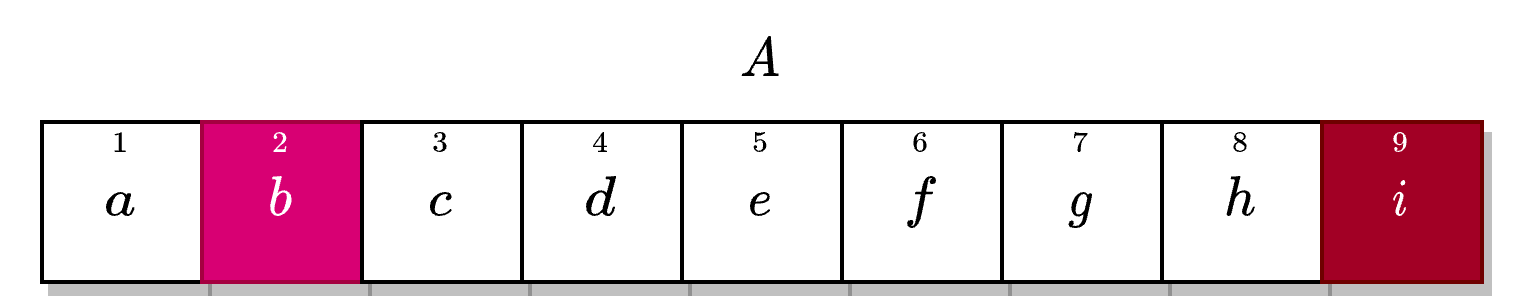
\includegraphics[width=0.75\linewidth]{assets/lec01-1d.png}
    \caption{Example 1}
\end{figure}

position 2 is a peak $\textit{iff}$ $b \ge a$ and $b \ge c$. 

For another, position 9 is a peak $\textit{iff}$ $i \ge h$. 

Find any peak(if it exists).

Link:\url{https://leetcode.com/problems/find-peak-element/}

\subsection{1D: Intuition}

Q: Does a peak always exist?

- if we change the definition into "A peak element is an element that is strictly greater than its neighbors", the argument doesn't hold anymore.

- Otherwise, peak always exists. \newline

We may imagine that $A[0] = A[n+1] = - \infty$, based on description.
- Perspective 1: Draw A Function/Curve

- Perspective 2: Greedy Ascent Algorithm

- Perspective 3: $-\infty$ suffices, then what about necessity?

\subsection{1D: Algorithm}

An Algorithm with $\Theta(\log_2^n)$ complexity

Strategy: Divide and Conquer (and Combine)

1. Divide the problem into disjoint subproblems(smaller instances of the same problem).

2. Conquer the subproblems by solving them recursively. 

3. Combine the solutions to the subproblems into the solution for the original problem.\newline

Procedure: Peek-Finding in $[1, n]$:

- if $n = 1$, n is one peak

- if $a[n/2-1] > a[n/2]$, Peek-Finding in $[1, n/2-1]$;

- else if $a[n/2+1] > a[n/2]$, Peek-Finding in $[n/2+1, n]$;

- else $n/2$ is one peak.

\begin{figure}[htbp]
    \centering
    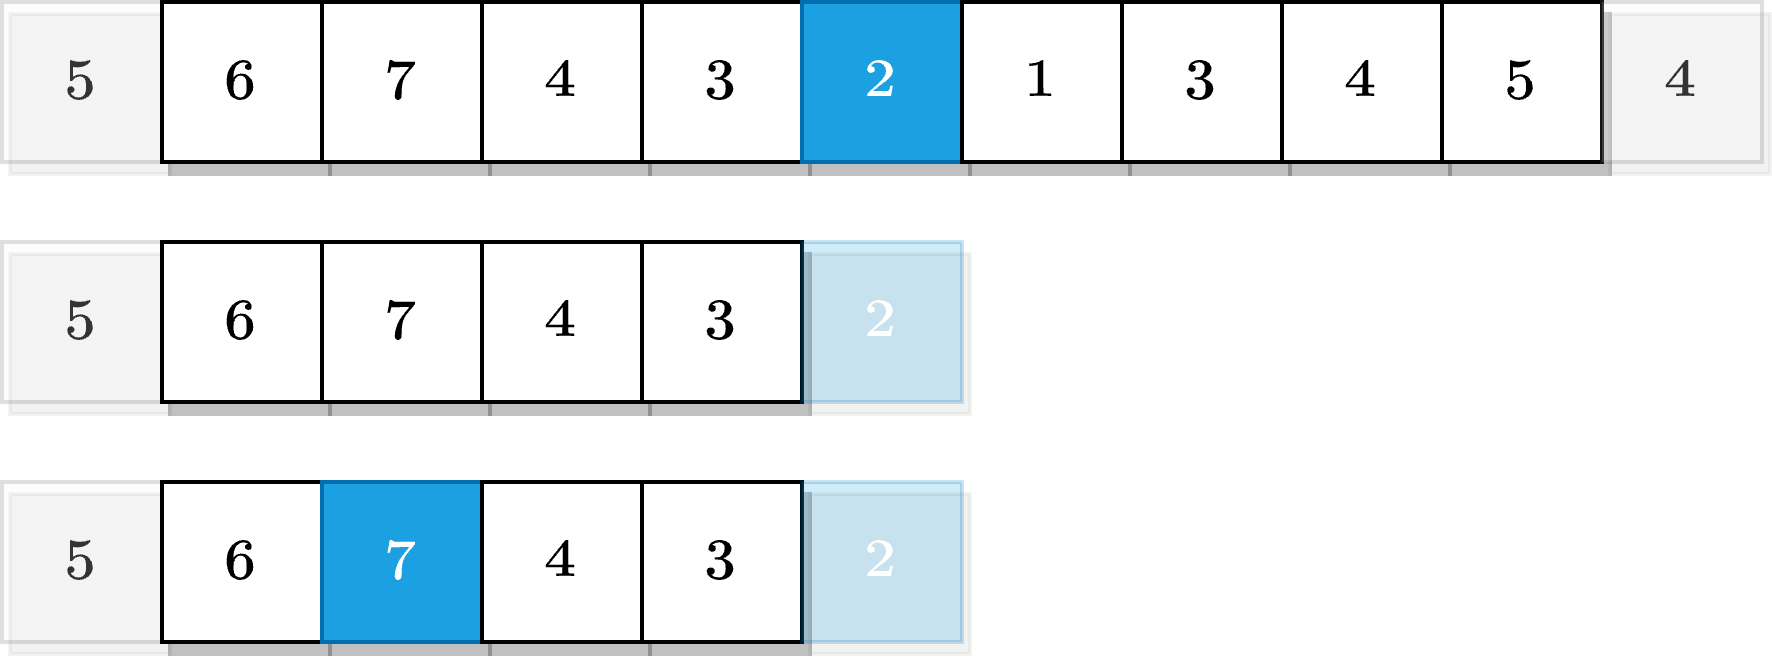
\includegraphics[width=0.75\linewidth]{assets/lec01-1d-eg2.png}
    \caption{Example 2}
\end{figure}

\subsection{2D: Problem}

A peak element in a 2D grid is an element that is no smaller than all of its adjacent neighbors to the left, right, top, and bottom.

In 2D case running on an grid of numbers, for example, 

$a$ is a peak $\textit{iff}$ $a \ge b$, $a \ge d$, $a \ge c$ and $a \ge e$. 

\begin{figure}[htbp]
    \centering
    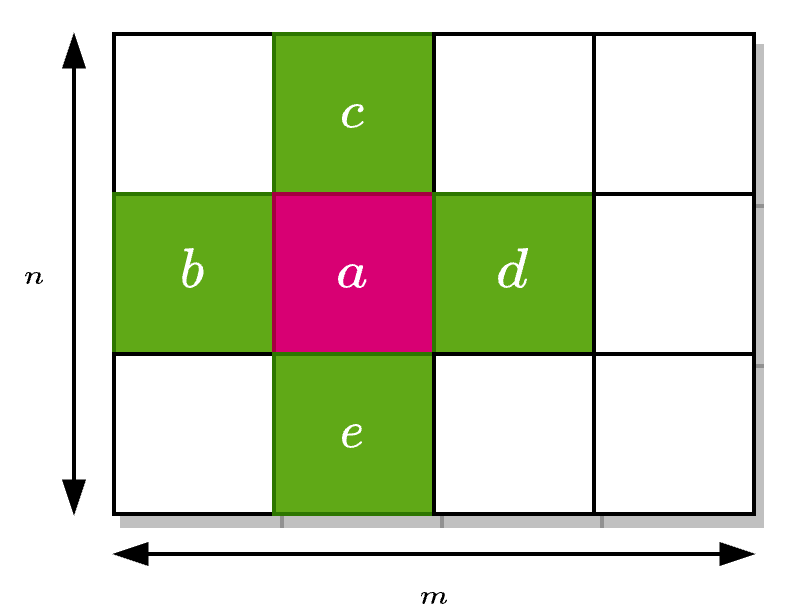
\includegraphics[width=0.25\linewidth]{assets/lec01-2d.png}
    \caption{Example 3}
\end{figure}

Link:\url{https://leetcode.com/problems/find-a-peak-element-ii/}

\subsection{2D: Intuition}

- if we change the definition into "A peak element is an element that is strictly greater than its neighbors", the argument doesn't hold anymore.

- Otherwise, a peak always exist. \newline

We may assume that the entire matrix is surrounded by an outer perimeter with the value $-\infty$ in each cell.

- Perspective 1: Conjure up an image of a Surface

- Perspective 2: Greedy Ascent Algorithm

- Perspective 3: $-\infty$ suffices, then what about necessity?

\subsection{2D: Algorithm}

\subsubsection{Attempt #1 with $\Theta(n m)$ complexity}

- For each column $j$, find its $\textit{global}$ maximum $B[j]$

- Apply 1D peak finder to find a peak (say $B[j]$) of $B[1...m]$

\begin{figure}[htbp]
    \centering
    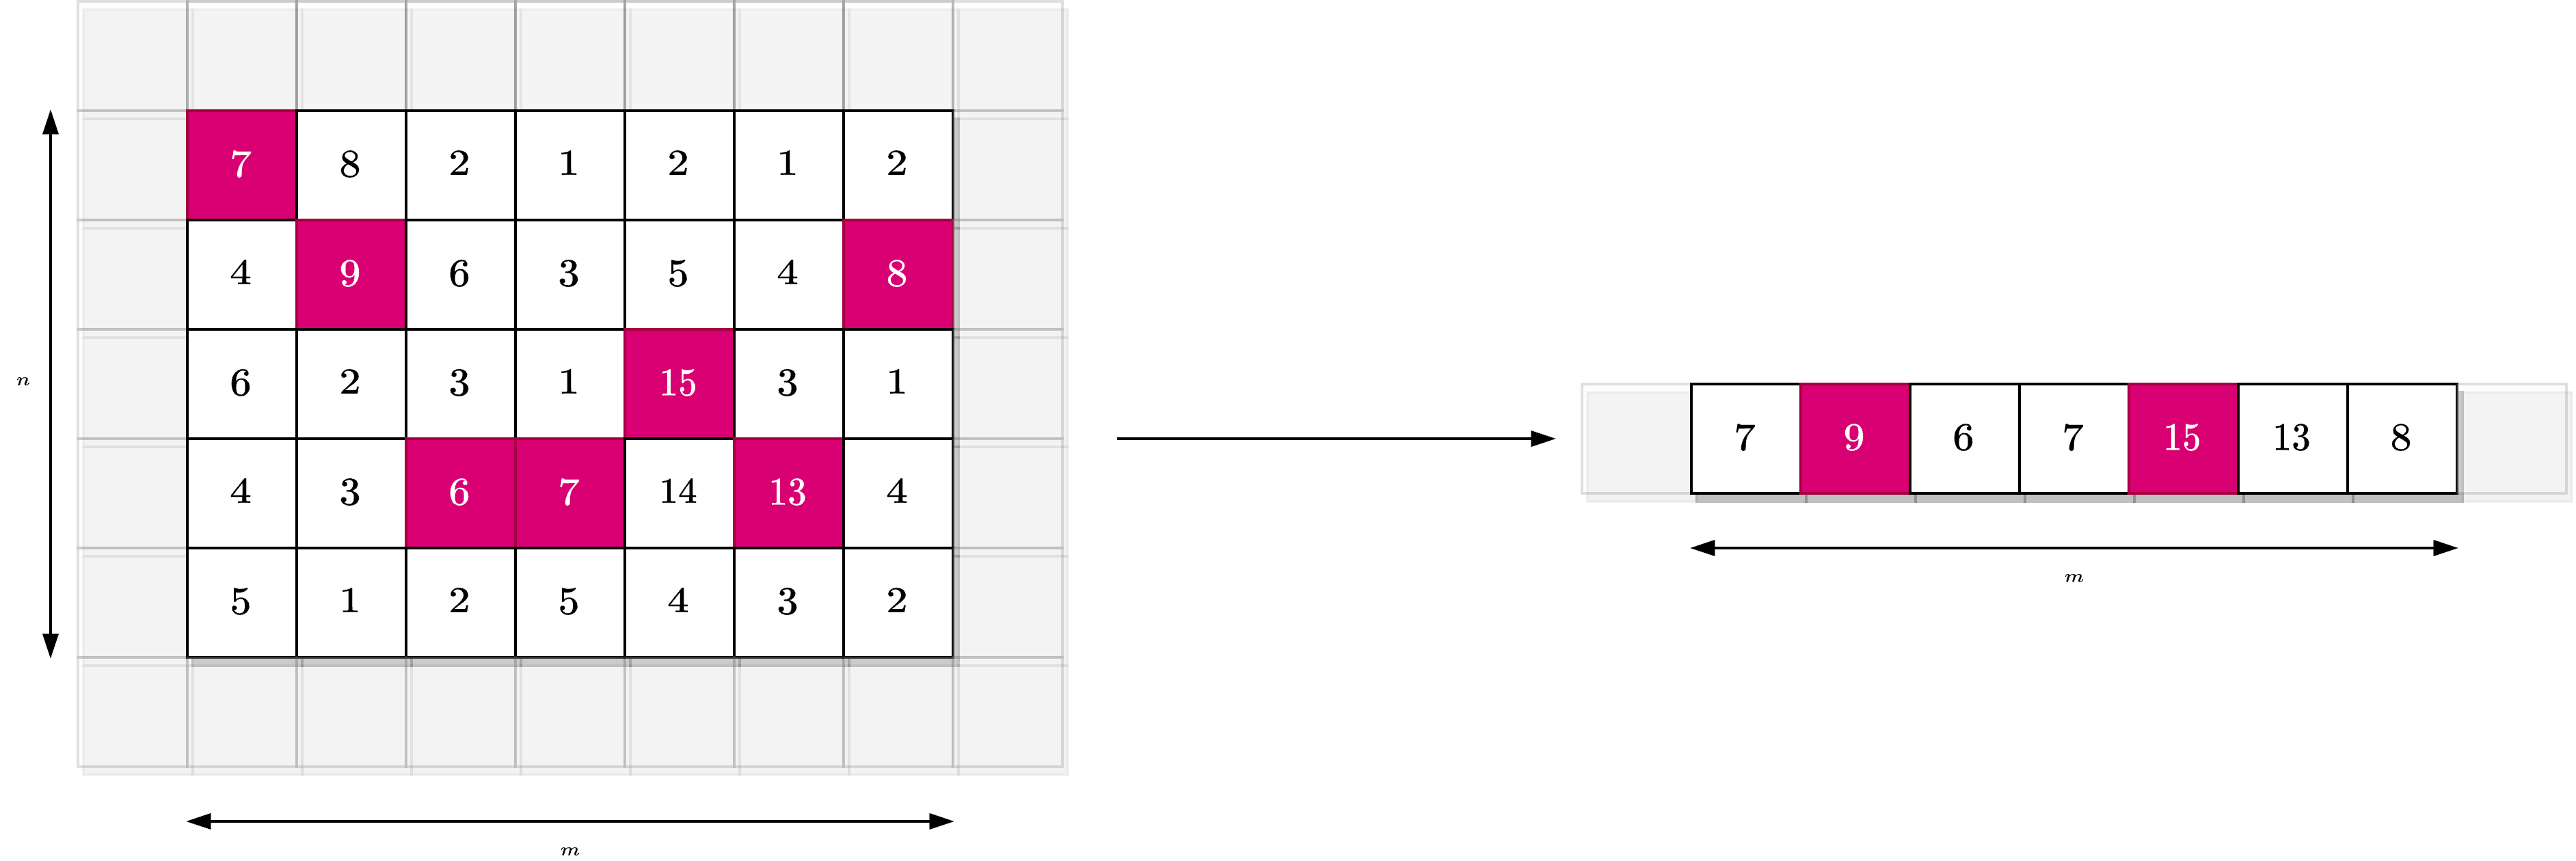
\includegraphics[width=0.9\linewidth]{assets/lec01-2d-eg.png}
    \caption{Example 3}
\end{figure}

\subsubsection{Attempt #2 with $\Theta(n\log_2^m)$ complexity}

1. Pick middle column ($j=m/2$)

2. Find $\textit{global}$ maximum $a=A[i,m/2]$in that column (and quit if $m=1$)

3. Compare $a$ to $b=A[i,m/2-1]$and $c=A[i,m/2+1]$

    - If $b>a$, recursion left columns
    
    - Else if $c>a$, then recursion right columns
    
    - Else $a$ is a 2D peak!


\begin{figure}[htbp]
    \centering
    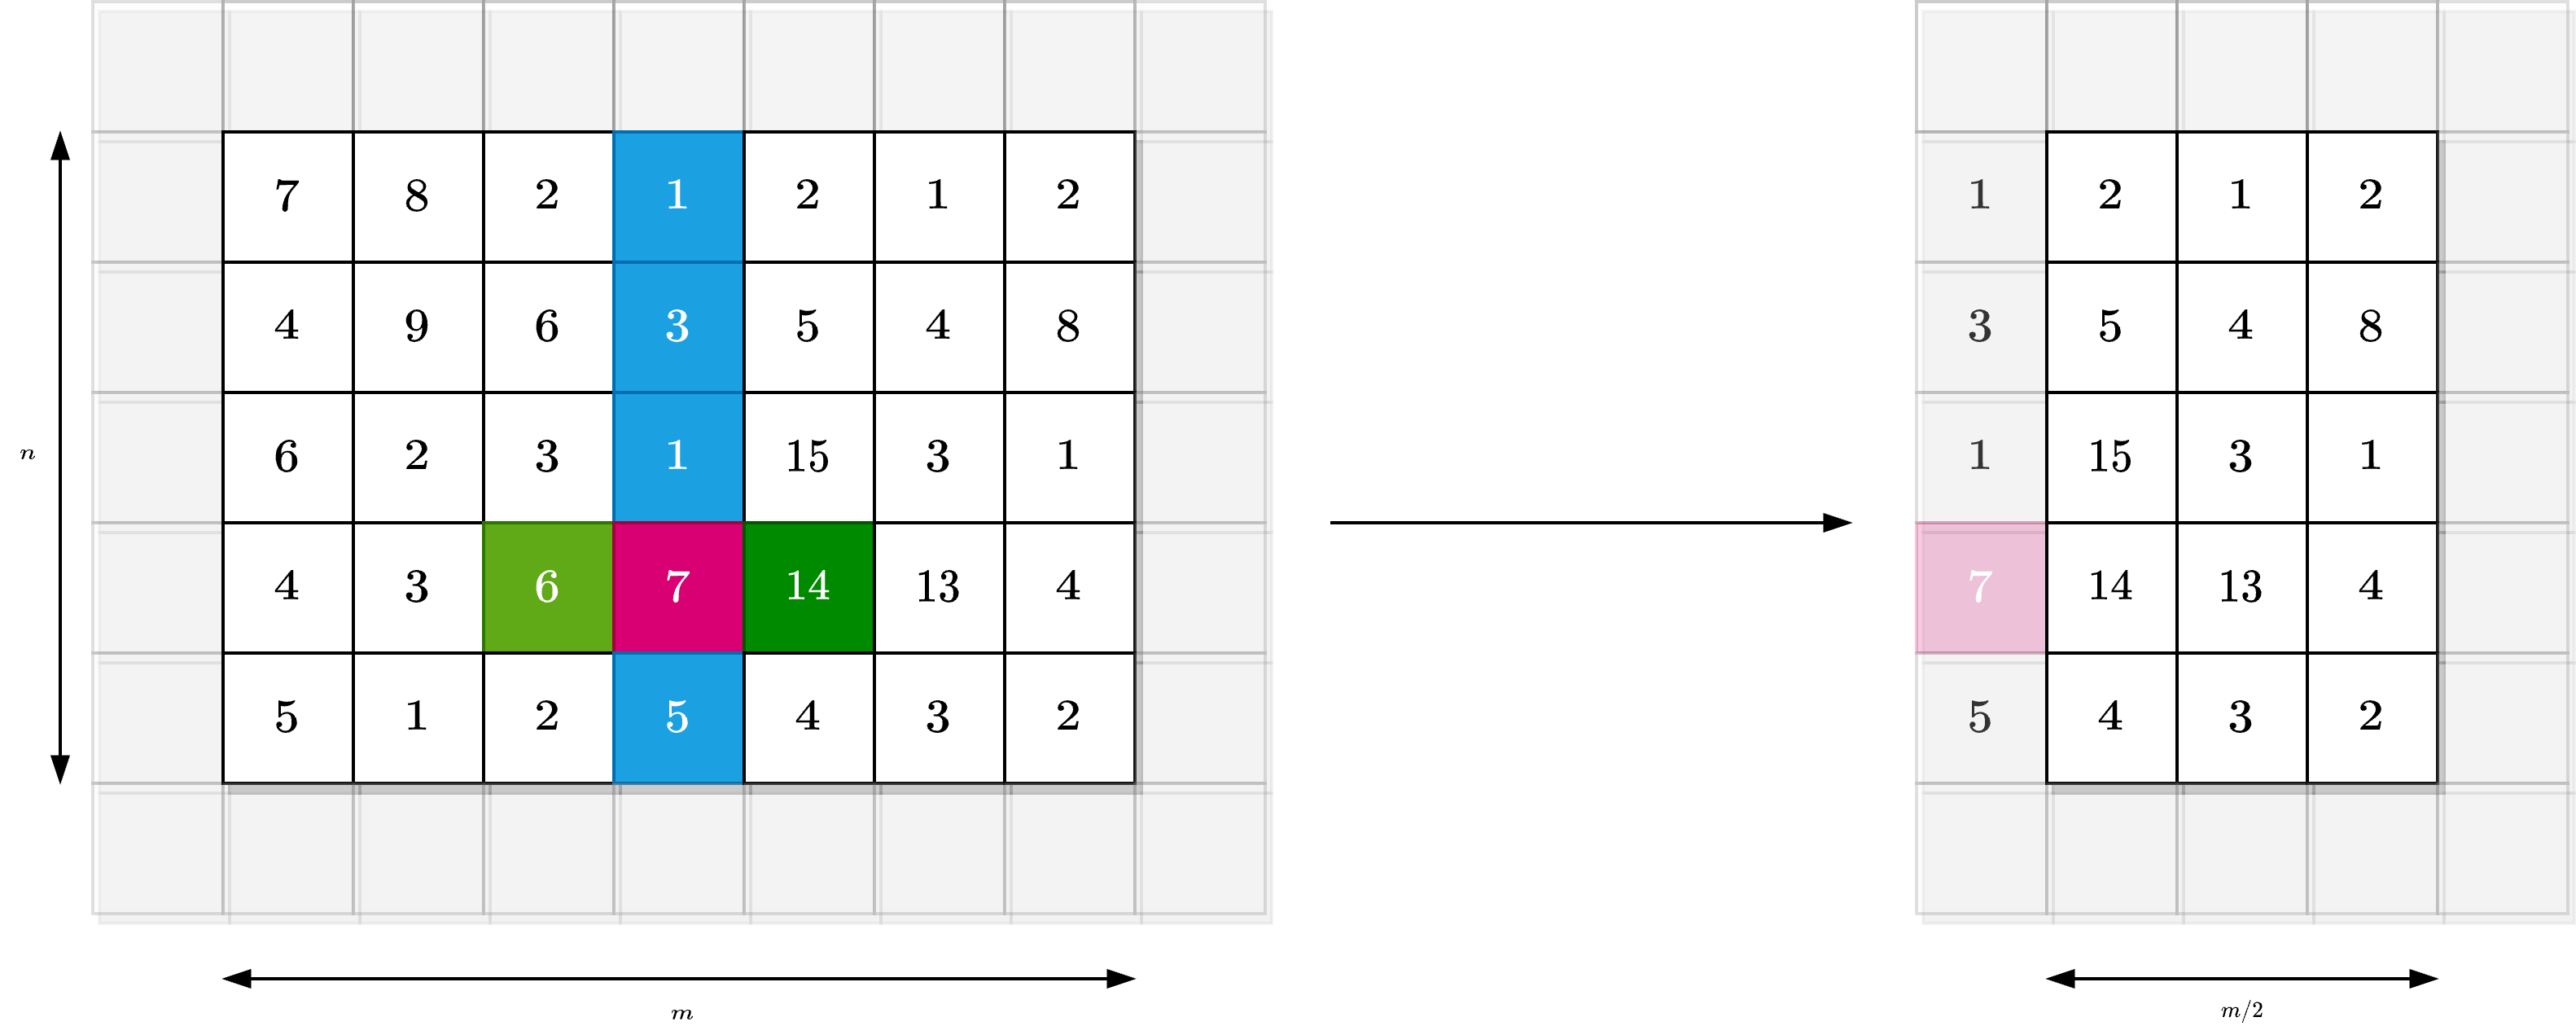
\includegraphics[width=0.98\linewidth]{assets/lec01-2d-eg2.png}
    \caption{Example 3}
\end{figure}

\subsubsection{Towards a linear-time algorithm}

- find global max on the cross

- if middle element done!

- o.w. two candidate sub-squares

- determine which one to pick by looking at its neighbors not on the cross\newline

\textbf{BUT: Not every peak of the chosen sub-square is necessarily
a peak of the large square. Hence, it is hard to recurse…}

\begin{figure}[htbp]
    \centering
    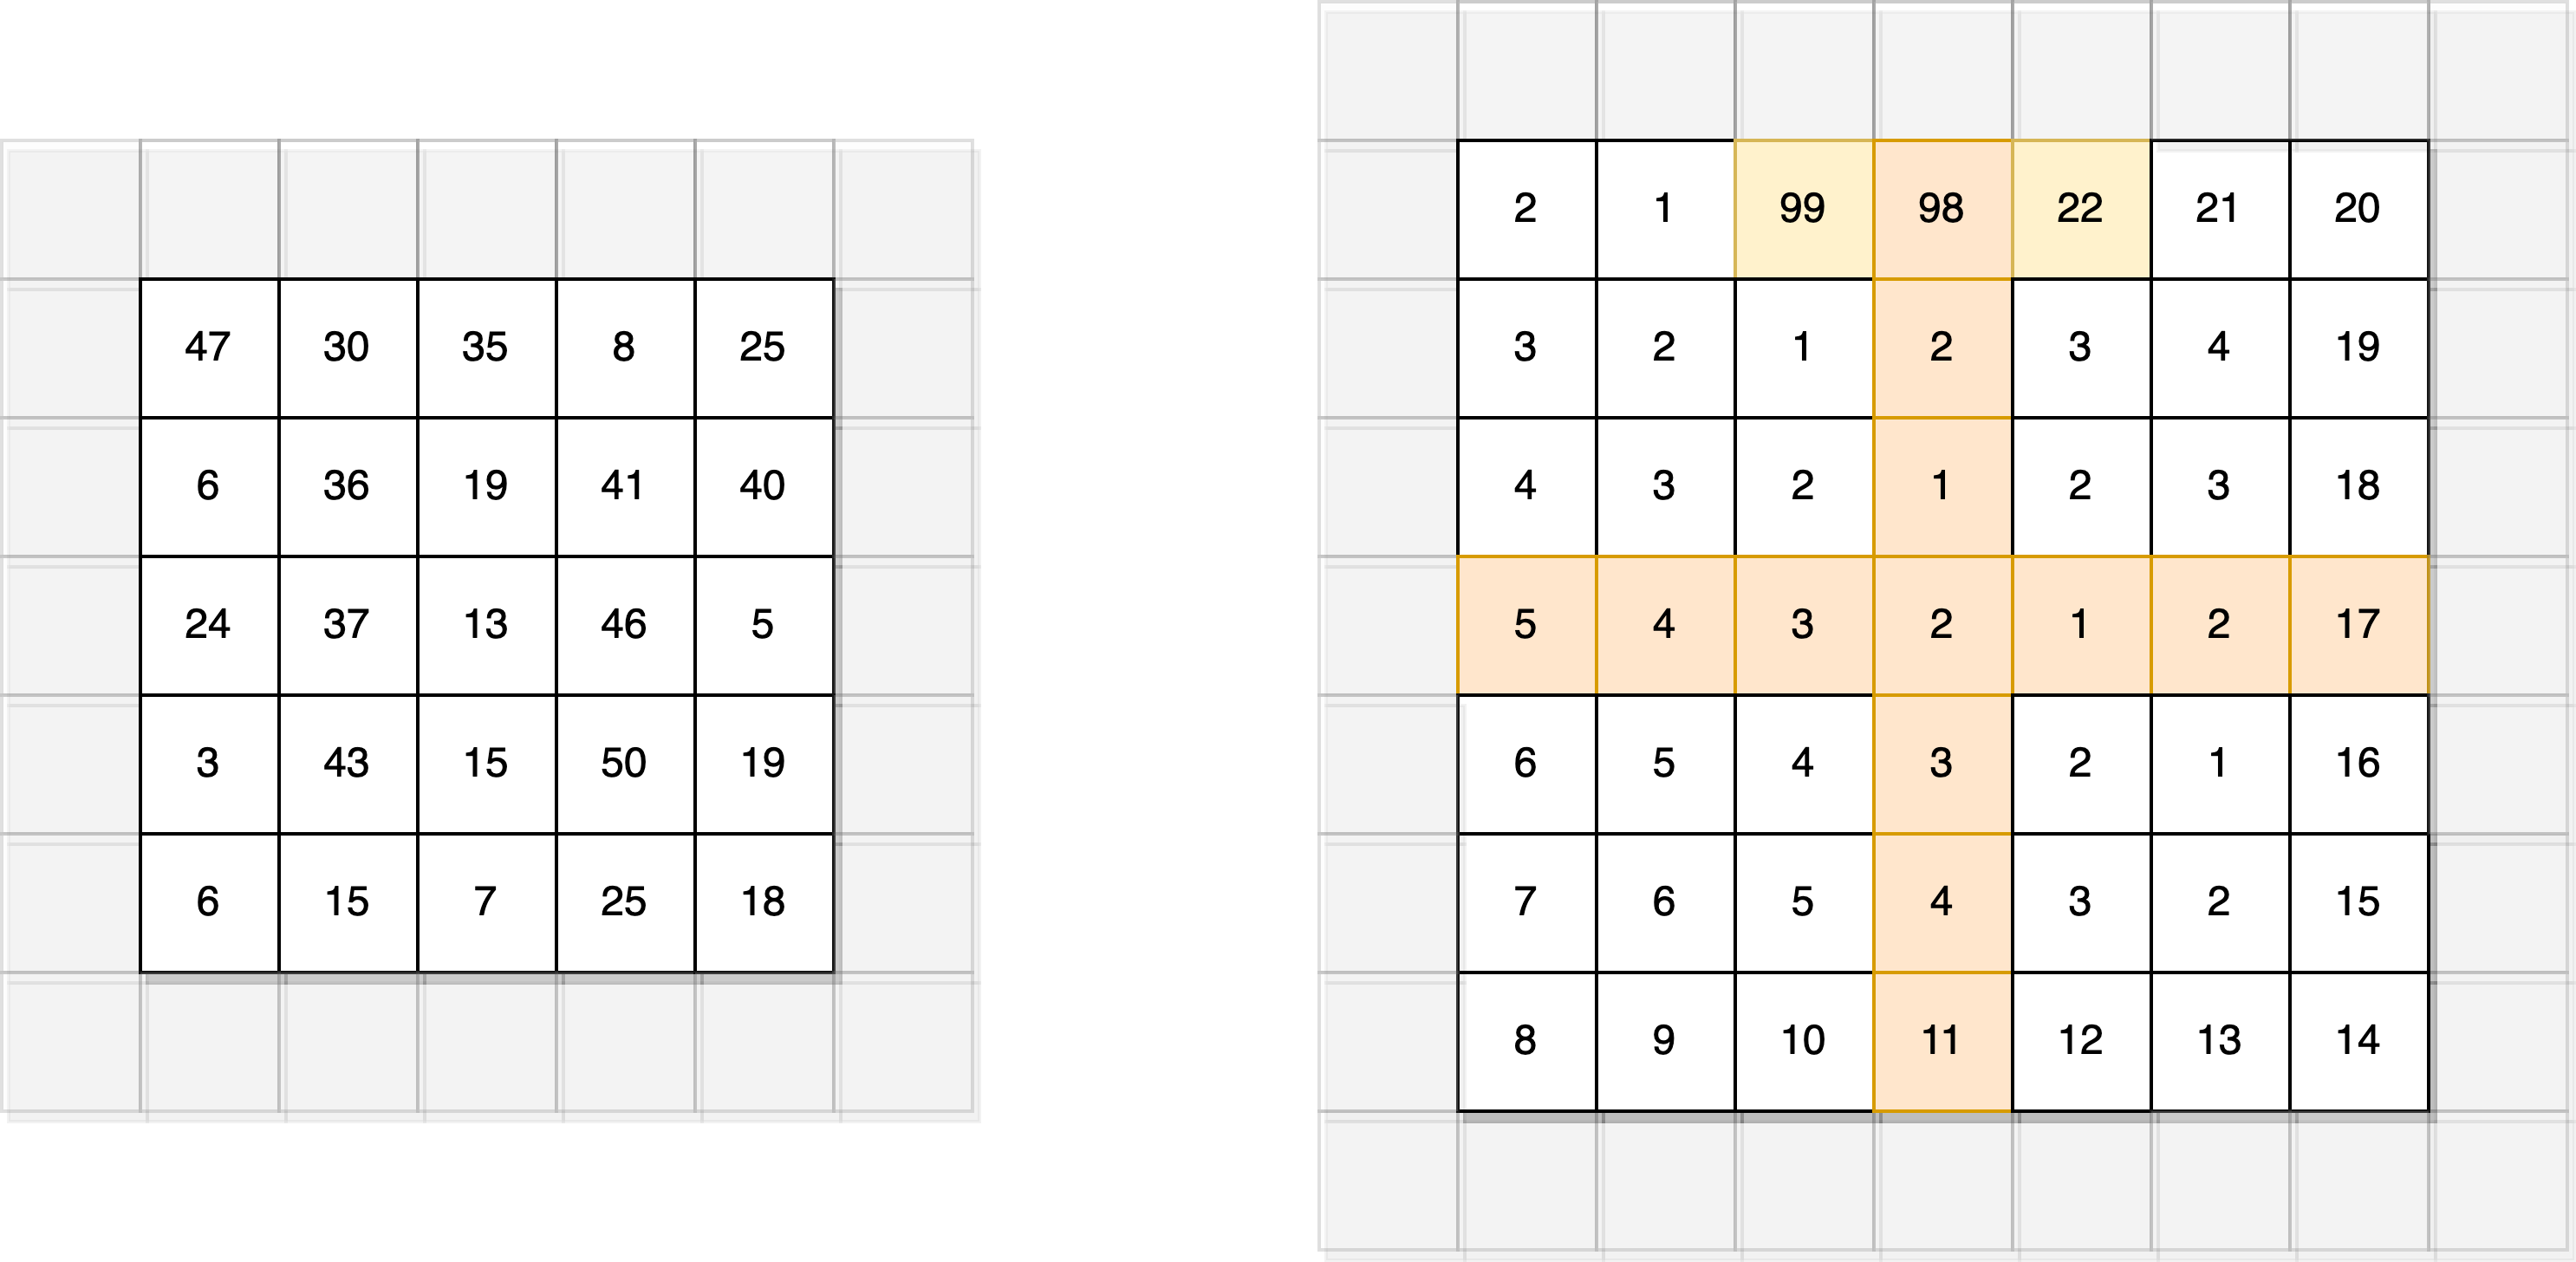
\includegraphics[width=0.88\linewidth]{assets/lec01-leetcode.png}
    \caption{A counter-example}
\end{figure}

\newpage
\section{作业}

\subsection{作业内容}
\begin{enumerate}
    \item 用Java语言完成全部例题,在Online Judge提交通过,提交代码、通过截图和调试过程过中遇到的问题和解决心得。
    \item 阅读欧拉计划货币面值的组合问题(见下附录),分析下面给出的各段代码的正误和时间复杂度。如果错误,给出一个反例并说明预期结果;如果正确,要用书面语体写出简要分析或证明。
    \item 以非递归形式编程实现Hanoi问题,要求输出搬动过程。
    \item (选做)峰值查找$O(n \text{log}n)$算法是否是最佳算法?如果是,请给出证明;如果不是,提出一个更好的做法并尝试给出正确性证明。
\end{enumerate}

\subsection{提交格式}

\subsection{附录:货币面值的组合问题}

提交链接:\url{https://www.luogu.com.cn/problem/U275899}

说明:下列代码改编自Java俱乐部成员孙嘉杰于2022年11月13日所作报告。

\newpage
\begin{lstlisting}[language={java},caption={Algorithm 1}]
public class Main {
    static int n = 200;
    static int[] coin = {1, 2, 5, 10, 20, 50, 100, 200};
    static Map<String, Integer> memo = new HashMap<>();

    public static int calcNumOfSolutions(int n, int maxCoinIdx) {
        // memo
        String key = n + " " + maxCoinIdx;
        if (memo.containsKey(key)) {
            return memo.get(n + " " + maxCoinIdx);
        }

        // terminal case
        if (maxCoinIdx <= 0) {
            return 1;
        }

        if (n < coin[maxCoinIdx]) {
            return calcNumOfSolutions(n, maxCoinIdx - 1);
        }

        // recursion
        memo.put(key, calcNumOfSolutions(n - coin[maxCoinIdx], maxCoinIdx) +
                calcNumOfSolutions(n, maxCoinIdx - 1));
        return memo.get(key);
    }

    public static void main(String[] args) {
        System.out.println(calcNumOfSolutions(n, coin.length - 1));
    }
}
\end{lstlisting}

\newpage
\begin{lstlisting}[language={java},caption={Algorithm 2}]
public class Main {
    static int n = 200;
    static int[] coin = {1, 2, 5, 10, 20, 50, 100, 200};
    static int[] memo = new int[n + 1];

    public static int calcNumOfSolutions(int n) {
        if (memo[n] != 0) {
            return memo[n];
        }

        int res = 0;
        for (int c : coin) {
            if (c <= n) {
                res += calcNumOfSolutions(n - c);
            }
        }
        memo[n] = res;
        return memo[n];
    }

    public static void main(String[] args) {
        memo[0] = 1;
        System.out.println(calcNumOfSolutions(n));
    }
}
\end{lstlisting}

\newpage
\begin{lstlisting}[language={java},caption={Algorithm 3}]
public class Main {
    static int n = 200;
    static int[] coin = {1, 2, 5, 10, 20, 50, 100, 200};
    static int[] memo = new int[n + 1];

    public static int calcNumOfSolutions(int n) {
        for (int i = 1; i < memo.length; i++) {
            for (int k : coin) {
                if (i >= k) {
                    memo[i] += memo[i - k];
                }
            }
        }
        return memo[n];
    }

    public static void main(String[] args) {
        memo[0] = 1;
        System.out.println(calcNumOfSolutions(n));
    }
}
\end{lstlisting}

\newpage
\begin{lstlisting}[language={java},caption={Algorithm 4}]
public class Main {
    static int n = 200;
    static int[] coin = {1, 2, 5, 10, 20, 50, 100, 200};
    static int[] memo = new int[n + 1];

    public static int calcNumOfSolutions(int n) {
        for (int k : coin) {
            for (int i = 1; i < memo.length; i++) {
                if (i >= k) {
                    memo[i] += memo[i - k];
                }
            }
        }
        return memo[n];
    }

    public static void main(String[] args) {
        memo[0] = 1;
        System.out.println(calcNumOfSolutions(n));
    }
}
\end{lstlisting}

\newpage
\begin{lstlisting}[language={java},caption={Algorithm 5}]
public class Main {
    static int n = 200;
    static int[] coin = {1, 2, 5, 10, 20, 50, 100, 200};
    static int[][] memo = new int[n + 1][coin.length];

    public static int calcNumOfSolutions(int n, int maxCoinIdx) {
        if (n < 0) {
            return 0;
        }
        if (memo[n][maxCoinIdx] != -1) {
            return memo[n][maxCoinIdx];
        }
        if (maxCoinIdx == 0) {
            return n % coin[0] == 0 ? 1 : 0;
        }
        int ans = calcNumOfSolutions(n - coin[maxCoinIdx], maxCoinIdx) + calcNumOfSolutions(n, maxCoinIdx - 1);
        memo[n][maxCoinIdx] = ans;
        return ans;
    }

    public static void main(String[] args) {
        Arrays.sort(coin);
        for (int i = 0; i <= n; ++i) {
            Arrays.fill(memo[i], -1);
        }
        System.out.println(calcNumOfSolutions(n, coin.length - 1));
    }
}
\end{lstlisting}

\end{document}

% \begin{table}[htbp]
%     \caption{常用的处理机调度策略}
%     \centering

%     \begin{threeparttable}
%         \begin{tabular}{cccccc}
%             \toprule
%             算法名称           & 主要适用范围       & 默认调度方式         \\
%             \midrule
%             先来先服务         & 作业调度\&进程调度 & 非抢占式             \\
%             短作业(进程)优先 & 作业调度\&进程调度 & 非抢占式             \\
%             高响应比优先       & 作业调度           & 非抢占式             \\
%             时间片轮转         & 进程调度           & 抢占式(不抢时间片) \\
%             多级反馈队列       & 进程调度           & 抢占式(抢占时间片) \\
%             \bottomrule
%         \end{tabular}

%         \zihao{-6}
%         \begin{tablenotes}
%             \item [*]   调度策略也就是调度算法
%         \end{tablenotes}

%     \end{threeparttable}
%     \qquad
% \end{table}

% \begin{figure}[htbp]
%     \centering
%     \includegraphics[height=550pt]{v1-class-compat.png}
%     \caption{UML类图(第二版)}
% \end{figure}

% \begin{minted}[mathescape,
%     linenos,
%     numbersep=5pt,
%     frame=lines,
%     gobble=4,
%     framesep=2mm]{Java}
%     public interface Observable {
%         void attachObserver(Observer o);

%         void detachObserver(Observer o);

%         void notifyObservers();
%     }
% \end{minted}

% \begin{lstlisting}[language={java},caption={收容队列(基于响应比的优先队列)}]
% private PriorityQueue<Task> queue = new PriorityQueue<>(new Comparator<Task>() {
%     @Override
%     public int compare(Task o1, Task o2) {
%         return (o2.getResponseRate(Clock.minutes) - o1.getResponseRate(Clock.minutes) > 0) ? (1) : (-1);
%     }
% });
% \end{lstlisting}